% --------------------------------------------------------------------------------------------------------------
%
% Copyright 2020-2023 Robert Bosch GmbH

% Licensed under the Apache License, Version 2.0 (the "License");
% you may not use this file except in compliance with the License.
% You may obtain a copy of the License at

% http://www.apache.org/licenses/LICENSE-2.0

% Unless required by applicable law or agreed to in writing, software
% distributed under the License is distributed on an "AS IS" BASIS,
% WITHOUT WARRANTIES OR CONDITIONS OF ANY KIND, either express or implied.
% See the License for the specific language governing permissions and
% limitations under the License.
%
% --------------------------------------------------------------------------------------------------------------
\section{System Overview}

\begin{figure}[htbp]
    \centering
    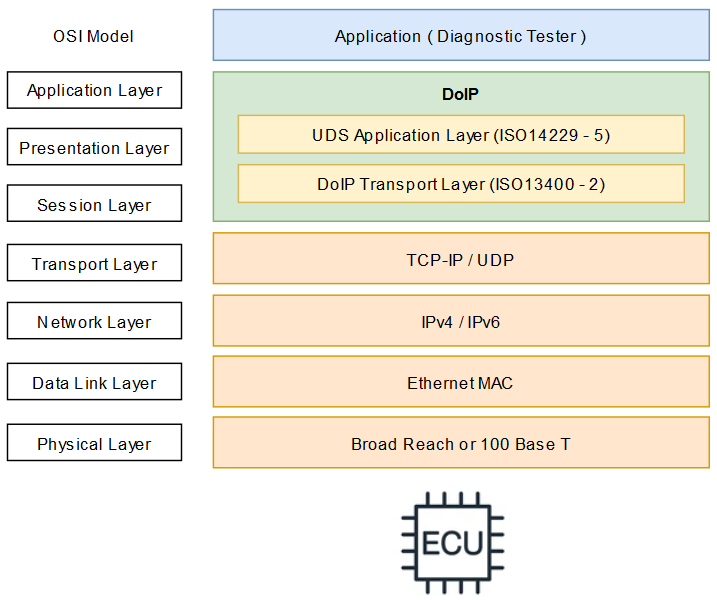
\includegraphics[width=0.8\textwidth]{./pictures/systems-overview.png}
    \caption{System overview}
    \label{fig:2.2}
\end{figure}

\begin{itemize}

\item The DoIP (Diagnostics over Internet Protocol) protocol is a standard for vehicle diagnostics that allows communication 
between diagnostic tester devices and electronic control units (ECU) over Ethernet networks.

\item DoIP is a standardized diagnostic transport protocol according to ISO 13400.
    \begin{itemize}

    \item DoIP Transport Layer (ISO 13400-2) is equipped with features to establish and maintain connection between external 
    tester device and DoIP gateway inside the vehicle.
    
    \item UDS application layer (ISO 14229-5) is the application profile that implements UDS on IP.

    \end{itemize}

\item The overall goal of the protocol is to encapsulate diagnostics messages of protocol standards like Unified Diagnostic Services (UDS)
and route them to and from the ECU.

\item The DoIP gateway or server can be a part of the ECU. A vehicle can have multiple DoIP entities and multiple testing devices and 
ECUs can route their traffic via a single DoIP entity. 

\item DoIP uses both User Datagram Protocol (UDP) and Transmission Control Protocol (TCP) for specific phases of the underlying layer. 
The initial announcement and identification messages are over UDP, after which the communication switches over to TCP.

\end{itemize}



% --------------------------------------------------------------------------------------------------------------
\section{DoIP application scenarios}

This section will provide some features along with examples through system above:
\begin{itemize}

    \item Vehicle identification and announcement: Is necessary to detect who is participating in the DoIP communication.

    \item Request diagnostic message: Request for diagnostic information, which is crucial for diagnosing vehicle issues 
    and ensuring effective communication within the DoIP network.

    \item Routing Activation: Allows that single Diagnostic Message pathes are activated or not to treat different protocols 
    different (like UDS and OBD) and to also treat single testers different.
        
    \item Entity DoIP (Gateway): Provides general information of the single DoIP entity. Usually used by the testers to get the
     current DoIP protocol relevant information from the single DoIPEntities.

    \item Alive mechanism: Is used to maintain different tester connections.

\end{itemize}

    % ---------------------------------------------
    \subsection{Example of Diagnostic Process}

        % ---------------------------------
        \subsubsection{Vehicle Diagnostics}

            \begin{figure}[htbp]
                \centering
                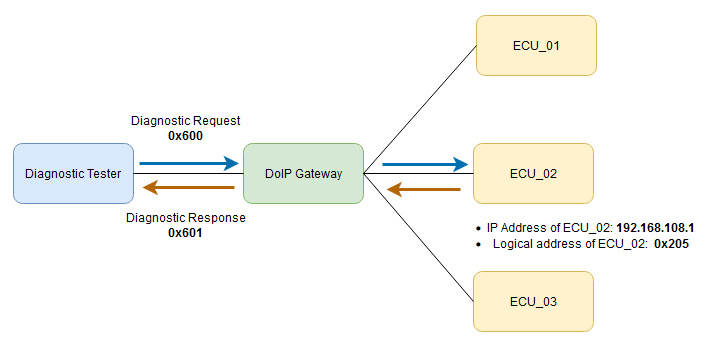
\includegraphics[width=0.8\textwidth]{./pictures/demo-vehicle-diagnostic.png}
                \caption{Vehicle diagnostic process demonstration}
                \label{fig:2.3}
            \end{figure}

            \begin{itemize}
                \item\textbf{Use Case:}\\
                    A vehicle diagnostic tool needs to establish a DoIP connection to communicate with an Electronic Control Unit (ECU)
                    within a vehicle for diagnostic purposes.

                \item\textbf{Scenario:} \\
                    The diagnostic tool initiates a connection to the ECU's IP address (192.168.108.1) and logical address 517 (0x205) using 
                    the \pkg\ library. \\
                    It sends a diagnostic message (600) to the ECU, receives a response, logs the response 
                    to the console, and then disconnects from the ECU.
            \end{itemize}

        \begin{robotcode}
*** Settings ***
Library    RobotFramework_DoIP

*** Test Cases ***
Test Establish an DoIP connection
    # Establish an connection to ecu ip address and ecu logical address
    Connect To ECU     192.168.108.1      517
    Send Diagnostic Message     600
    ${res}= Receive Diagnostic Message
    Log To Console    ${resp}
    Disconnect
        \end{robotcode}

        % ---------------------------------
        \subsubsection{Remote Testing}
            \begin{figure}[htbp]
                \centering
                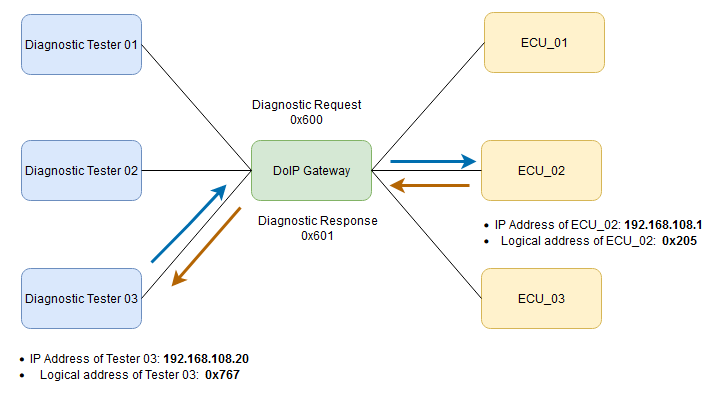
\includegraphics[width=0.8\textwidth]{./pictures/demo-remote-diagnostic.png}
                \caption{Remote diagnostic process demonstration}
                \label{fig:2.3}
            \end{figure}

            \begin{itemize}
                \item\textbf{Use Case:}\\
                    A remote testing environment requires a connection between a target tester and an ECU located in a different location.

                \item\textbf{Scenario:} \\
                    The target tester, located at IP address 192.168.108.20, establishes a DoIP connection to the ECU at IP address 192.168.108.1 
                    and logical address 517 (0x205). Additionally, the target tester specifies its own logical address 1895 (0x767) using the \pkg\ 
                    library. \\
                    It sends a diagnostic message (600) to the ECU, receives a response, logs the response to the console, and then disconnects 
                    from the ECU.
            \end{itemize}

            \begin{robotcode}
*** Settings ***
Library    RobotFramework_DoIP

*** Test Cases ***
Test Establish an DoIP connection between specific tester and target ECU 
    # Establish an connection to ecu ip address and ecu logical address
    Connect To ECU     192.168.108.1      517       client_ip_address=192.168.108.20    client_logical_address=1895
    Send Diagnostic Message     600
    ${res}= Receive Diagnostic Message
    Log To Console    ${resp}
    Disconnect
            \end{robotcode}

    % ---------------------------------------------
    \subsection{Example of Vehicle Identification}
        \begin{itemize}
            \item\textbf{Use Case:}\\
                A diagnostic tool needs to request vehicle identification information from an Electronic Control Unit (ECU) within a vehicle.

            \item\textbf{Scenario:} \\
                The diagnostic tool initiates a DoIP connection to the ECU's IP address (192.168.108.1) and logical address (205) using the 
                \pkg\ library. It then sends a request for vehicle identification information to the ECU.
        \end{itemize}

        \begin{robotcode}
*** Settings ***
Library    RobotFramework_DoIP

*** Test Cases ***
Test Request Vehicle Identification
    Connect To ECU     192.168.108.1      205
    Request Vehicle Identification 

        \end{robotcode}

% --------------------------------------------------------------------------------------------------------------

